\documentclass[a4paper,10pt]{article}
\usepackage[utf8]{inputenc}
\usepackage{graphicx}

\title{Calculation of the first cosmic velocity}
\author{Timofei Ryko}

\begin{document}

\maketitle
When we talk about motion along the Earth's orbit (we will assume that this is motion along a circle), centripetal acceleration can be taken as g. So, firsty it is good idea to come up with a formula for centripetal acceleration.
\par
Let's look at the movement of the body in a circle for a short period of time (figure \ref{fig:1}). Let's draw the displacement vector, as well as the velocity vectors in the initial and final velocity. To find the change in velocity, we subtract the last two vectors from each other.
\begin{figure}[h]
    \centering
    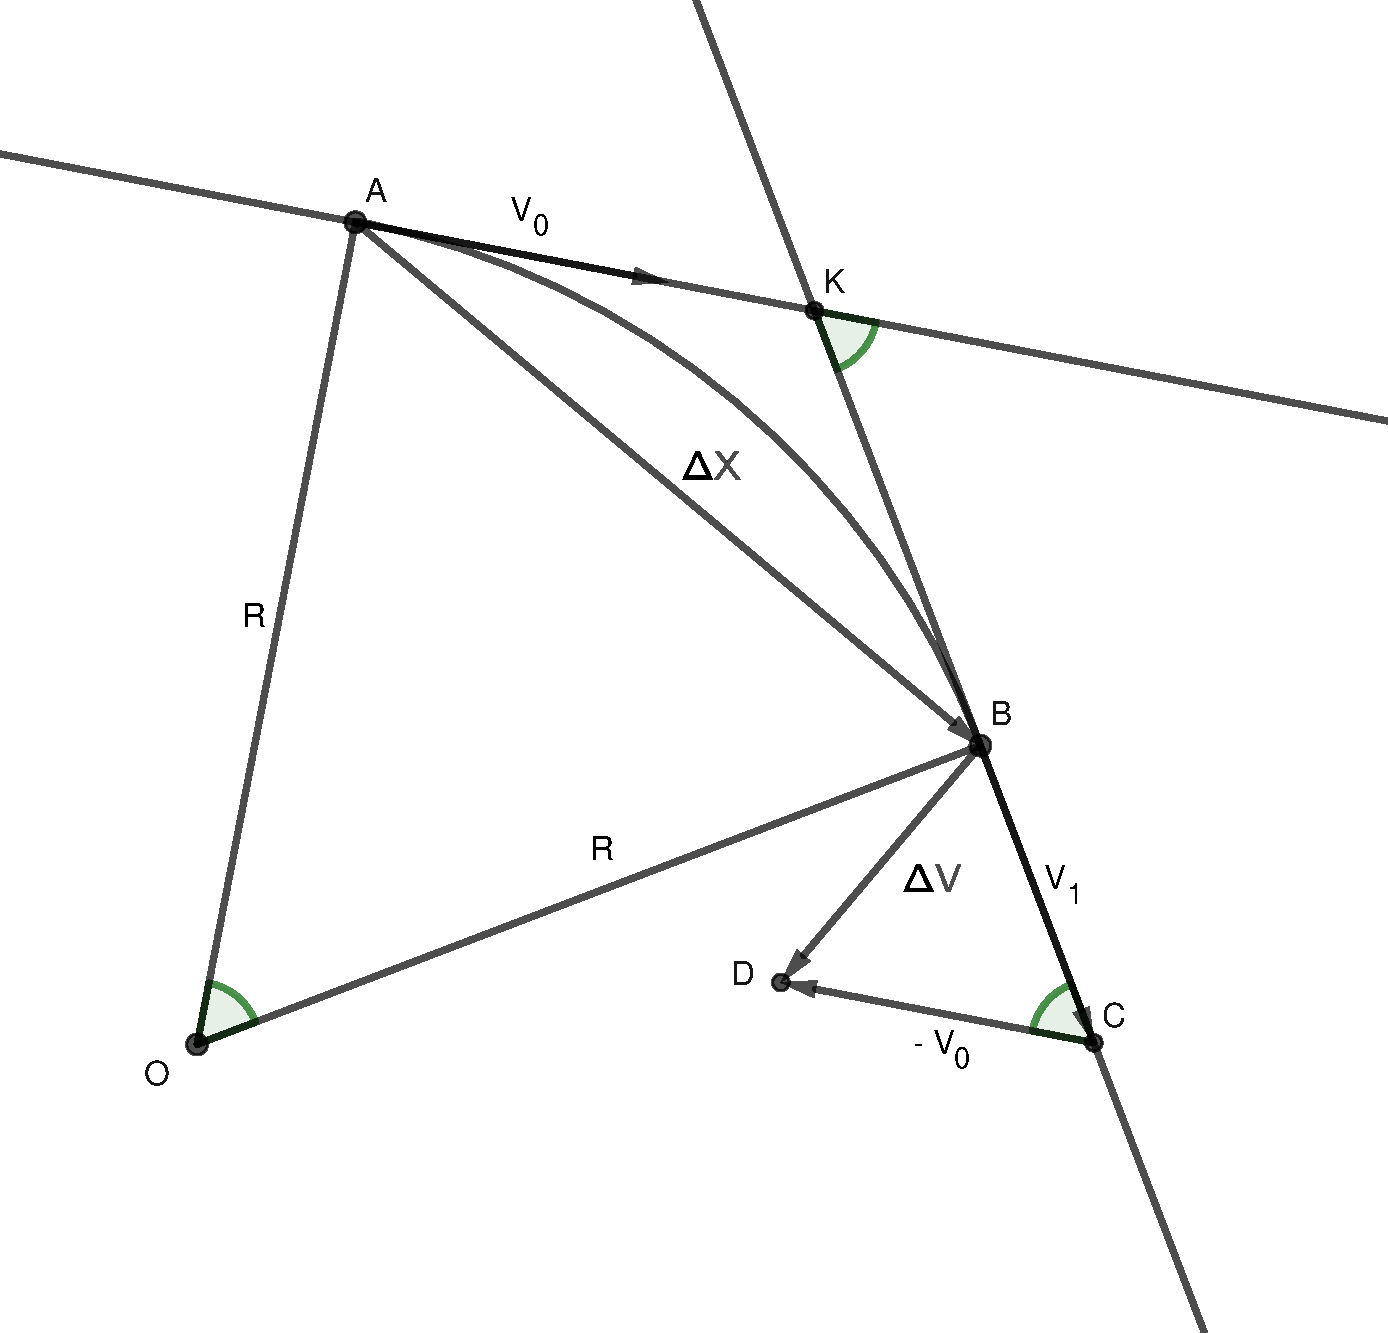
\includegraphics[width=1\textwidth,
    trim={1cm 1cm 1cm 1cm},clip]{figure.pdf}
    \caption{A small sector of the circle, velocity and displacement vectors.}
    \label{fig:1}
\end{figure}
\newpage
\par
$\angle BCD = 180^{\circ} - \angle AKB$
\par
The tangents are $\perp$ to the radiuses, so
\par
$\angle AKB = 360^{\circ} - 2 \cdot 90^{\circ} - \angle AOB =
180^{\circ} - \angle AOB$
\par
$=> \angle BCD = 180^{\circ} - 180^{\circ} + \angle AOB = \angle AOB$
\par
Triangles AOB and BCD are isosceles, so they have all other angles equal
\par
$=> \triangle AOB \sim \triangle BCD$
\par
It means, that $\Delta v / v = \Delta x / R$ (the sector is small so we can say that the path in a straight line is equal to the path in an arc). Dividing this expression by time, we get:
\begin{center}
\[ \scalebox{1.75}{$\frac{a}{v} = \frac{v}{R} => a = \frac{v^2}{R}$} \]
\end{center}
We can also come up with such formula more formally, using limits: let's say that $\Delta y$ is the changing the coordinate along the axis tangent to the circle and $\Delta z$ is the changing the coordinate along the axis perpendicular to the tangent, that is, parallel to the radius:
\begin{center}
\[ \scalebox{1}{$R^2 + \Delta y^2 = (R + \Delta z)^2$} \]
\[ \scalebox{1}{$\Delta y = \sqrt{\Delta z^2 + 2R\Delta z}$} \]
\[ \scalebox{1}{$\Delta z = at^2 / 2, \Delta y = vt = v\sqrt{2\Delta z / a}$} \]
\[ \scalebox{1}{$\lim_{\Delta z\to 0} v = \sqrt{\frac{a(2R + \Delta z)}{2}} = \sqrt{aR}$} \]
\end{center}
Returning to the task, now it is easy to calculate the first cosmic velocity:
\begin{center}
\[ \scalebox{1.5}{$v = \sqrt{gR}$} \]
\end{center}
In case the body is launched close to the surface of the Earth, $R = 6.371 \cdot 10^6 m$:
\begin{center}
\[ \scalebox{1.5}{$v = \sqrt{9.8 \cdot m \cdot s^{-2} \cdot 6.371 \cdot 10^6 \cdot m} = 7901 \cdot m \cdot s^{-1}$} \]
\end{center}
However, in real life, satellites orbit the earth at a sufficiently high altitude and it must be taken into account. For example, for the International Space Station, the rotation speed will be as follows:
\begin{center}
\[ \scalebox{1.5}{$v = \sqrt{9.8 \cdot m \cdot s^{-2} \cdot 6.773 \cdot 10^6 \cdot m} = 8147 \cdot m \cdot s^{-1}$} \]
\end{center}
Solving this task we did not take into account, that in reality orbit can be not a circle, the force of gravity decreases with distance from the earth and other factors. Nevertheless, we were able to give a fairly accurate estimate.
\end{document}
